% Correct rates with Wilson 95% intervals for the tuned set and the five clean held-out runs.
% x = (percent - 60) * 0.3 cm, so the axis spans 60 to 95 percent over 10.5 cm.
\begin{figure}[htbp]
\centering
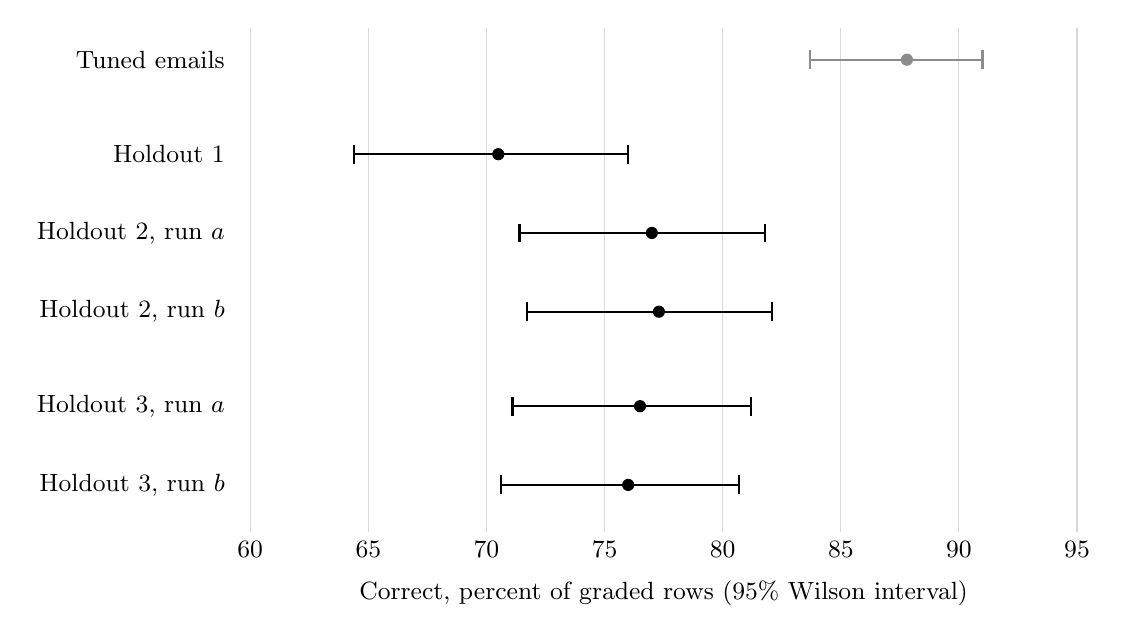
\begin{tikzpicture}[x=1cm,y=1cm,font=\small]
  \foreach \p in {60,65,70,75,80,85,90,95} {
    \draw[black!15] ({(\p-60)*0.3},0.4) -- ({(\p-60)*0.3},-6.0);
    \node[below] at ({(\p-60)*0.3},-6.0) {\p};
  }
  \node[below] at (5.25,-6.5) {Correct, percent of graded rows (95\% Wilson interval)};
  \foreach \y/\lab/\lo/\pt/\hi/\sty in {
      0/Tuned emails/83.7/87.8/91.0/black!45,
     -1.2/Holdout 1/64.4/70.5/76.0/black,
     -2.2/{Holdout 2, run $a$}/71.4/77.0/81.8/black,
     -3.2/{Holdout 2, run $b$}/71.7/77.3/82.1/black,
     -4.4/{Holdout 3, run $a$}/71.1/76.5/81.2/black,
     -5.4/{Holdout 3, run $b$}/70.6/76.0/80.7/black} {
    \node[left,align=right] at (-0.2,\y) {\lab};
    \draw[\sty,line width=.8pt] ({(\lo-60)*0.3},\y) -- ({(\hi-60)*0.3},\y);
    \draw[\sty,line width=.8pt] ({(\lo-60)*0.3},\y-0.12) -- ({(\lo-60)*0.3},\y+0.12);
    \draw[\sty,line width=.8pt] ({(\hi-60)*0.3},\y-0.12) -- ({(\hi-60)*0.3},\y+0.12);
    \fill[\sty] ({(\pt-60)*0.3},\y) circle (2.2pt);
  }
\end{tikzpicture}
\caption[Correct rates of the deployed agent on the tuned emails and on the five clean held-out runs, with Wilson 95 percent intervals]{Correct rates of the deployed agent on the tuned emails and on the five clean held-out runs, with Wilson 95 percent intervals (a confidence interval for a percentage). The five clean runs were graded by Sonnet under the current rubric. The tuned emails (grey) were graded by Opus, supplied the fixes and are contaminated. The intervals of all clean runs overlap, while the tuned set lies higher.}
\label{fig:live-holdout}
\end{figure}
